\section{Typkompatibilität}\label{sec:typecompatibility}


Für die folgenden Beispiele sei in Java folgende Vererbungsbeziehung gegeben:

\begin{minted}[mathescape,
    gobble=2]{java}
    class A {
        public int x = 0;
        public void inA() {
            ...
        }
        public void whoAmI() {
            System.out.println("A");
        }
    }

    class B extends A {
        public int x = 1;
        public void inB() {
        }
        public void whoAmI() {
            System.out.println("B");
        }
    }
\end{minted}\\

\begin{itemize}
    \item Klasse \code{A} ist ein \code{java.lang.Object}
    \item Klasse \code{B} ist ein \code{A}
    \item Klasse \code{B} ist ein \code{java.lang.Object}
\end{itemize}

\subsection{Ersetzbarkeitsprinzip}

Immer dann, wenn ein bestimmter Typ gefordert wird, ist auch sein Untertyp erlaubt (vgl.~\cite[466]{Ull23})\footnote{
Der Kern des \textit{Liskovschen Substitutionsprinzip}, das in Abschnitt~\ref{subsec:covariance} näher beleuchtet wird
}.\\

\noindent
Der folgenden Methode kann ohne weiteres ein Objekt vom Typ \code{B} übergeben werden: Da \code{B} ein \code{A} ist,
hat es automatisch seine Methode \code{inA()} geerbt:

\begin{minted}[mathescape,
    gobble=2]{java}
    class C {
        public void foo(A a) {
            a.inA();
        }
    }
    C c = new C();
    B b = new B();
    c.foo(b);
\end{minted}\\

\subsection{Typumwandlung}

Wie \textit{Ullenboom} in ~\cite[467 f.]{Ull23} zeigt, ist für den Compiler der \textit{Referenztyp} wesentlich, für die Laufzeitumgebung hingegen der \textit{Objekttyp} (s. Abbildung~\ref{fig:types}).\\

\begin{figure}
    \begin{center}
        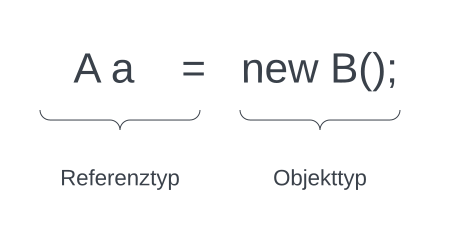
\includegraphics[scale=0.5]{chapters/OOP/img/types}
        \caption{Referenztyp und Objekttyp in Java.
        Der Compiler berücksichtigt vor allem den Referenztyp. (Quelle: in Anlehnung an~\cite[467 f., ``Begrifflichkeit``]{Ull23})}
        \label{fig:types}
    \end{center}
\end{figure}

\noindent
So kompiliert folgende Ausdrucksanweisung problemlos:

\begin{minted}[mathescape,
    gobble=2]{java}
    A a = new B();
\end{minted}\\

\noindent
Allerdings kann im folgenden Code nur auf Eigenschaften der Klasse \code{A} über die lokale Variable \code{a} zugegriffen werden - dass eigentlich ein Objekt vom Typ \code{B} in \code{a} steckt, interessiert den Compiler nicht:\\

\begin{minted}[mathescape,
    gobble=2]{java}
    A a = new B();
    a.inB(); // Fehler "Cannot resolve method 'inB' in 'A'"
\end{minted}\\

\begin{tcolorbox}
    Obwohl der Compiler die Methode \code{inB()} nicht auflösen kann, löst die Laufzeitumgebung problemlos den Typen
    von \code{a} zu \code{B} auf:
    \begin{minted}{java}
        A a = new B();
        System.out.println(a instanceof B); // true
    \end{minted}\\

    \noindent
    Auch, wenn der \textit{Compiler} nur Aufrufe zu Methoden der Klasse \code{A} auflösen kann,
    werden Methoden, die in \code{B} überschrieben werden, zur \textit{Laufzeit} auf \code{b} aufgerufen:

    \begin{minted}{java}
        A a = new B();
        System.out.println(a instanceof B); // true
        a.whoAmI();// "B"
    \end{minted}\\

\end{tcolorbox}\\

\begin{tcolorbox}[title={Felder werden überdeckt}]
    Felder werden in Java \textit{nicht} überschrieben.\\
    Enthält eine Unterklasse ein Feld gleichen Namens, überdeckt dieses Feld das Feld der Superklasse.\\
    Ein Zugriff auf das Feld der Superklasse ist von der Unterklasse nur über \code{super.[feldname]} möglich, oder über explizites Casting:
    \code{((Superklasse)this).[feldname]}.\\

    \noindent
    \blockquote[{\cite[505]{Ull23}}]{
    Bei Methodenaufrufen bindet das Laufzeitsystem immer dynamisch; bei Zugriffen auf Objektvariablen ist das nicht so: Hier bestimmt der Compiler,
    von welcher Klasse die Objektvariable genommen werden soll.
    }\\

    \noindent
    Aus diesem Grund liefert das folgende Programm als Ausgabe zunächst $0$.
    Erst ein explizites casten ermöglicht den Zugriff auf die in der Unterklasse überdeckte Eigenschaft, worauf die Ausgabe $1$ erfolgt:

    \begin{minted}{java}
        A a = new B();
        System.out.println(a.x); // "0", weil in B überdeckt.
        System.out.println(((B)a).x); // "1"
    \end{minted}

\end{tcolorbox}

\noindent
Um dennoch auf \code{inB()} zugreifen zu können, kann \code{a} explizit nach \code{B} gecasted werden.\\

\noindent
I.d.R. wird der Compiler aufgrund erkannter Typinkompatibilität das Kompilieren verhindern; werden durch den Compiler diese Inkompatibilitäten aber nicht erkannt, wird die Laufzeitumgebung veranlasst, die Operation durchzuführen - gelingt das nicht, wird eine \code{ClassCastException}\footnote{
``Class ClassCastException``: \url{https://docs.oracle.com/en/java/javase/21/docs/api/java.base/java/lang/ClassCastException.html} - abgerufen 07.03.2024
} geworfen, die folgerichtig eine Exception vom Typ \code{RuntimeException} ist\footnote{
Abschnitt ~\ref{ch:exceptions} widmet sich etwas ausführlicher den Eigenschaften von Laufzeit-Ausnahmen.
}:

\begin{minted}[mathescape,
    gobble=2]{java}
    Object a = new B();
    String s = (String)a; // ClassCastException
\end{minted}\\

\noindent
Die eben erwähnte Typumwandlung funktioniert letztendlich durch explizites casting wie folgt:

\begin{minted}[mathescape,
    gobble=2]{java}
    A a = new B();
    ((B)a).inB();
\end{minted}\\

Eine implizite Typumwandlung kann durch eine explizite ersetzt werden\footnote{
    je nach Entwicklungsumgebung wird an dieser Stelle der Hinweis gegeben, dass dies bereits durch den Compiler geschieht.
}:

\begin{minted}[mathescape,
    gobble=2]{java}
    B b = new B();
    A a = (A)b;
    Object o = (Object)a;
\end{minted}\\

\noindent
Explizites casting funktioniert nicht zum spezielleren Typ:

\begin{minted}[mathescape,
    gobble=2]{java}
    A a = new A();
    B b = (B)a; // ClassCastException
\end{minted}\\


\subsection{Kovarianz}\label{subsec:covariance}
Sobald es sich bei dem Rückgabetyp einer Methode um einen \textit{Referenztypen} handelt, muss der Rückgabetyp der Methode in der Unterklasse folgende Bedingung erfüllen\footnote{
    vgl. ``Java Language Specification - 8.4.8.3. Requirements in Overriding and Hiding``: \url{https://docs.oracle.com/javase/specs/jls/se21/html/jls-8.html#jls-8.4.8.3}
}:

\begin{itemize}
    \item Der Rückgabetyp der Methode in der Unterklasse muss \textbf{kovariant} zu dem Rückgabetyp der überschriebenen Methode sein\footnote{
        vgl. ``Java Language Specification - 8.4.5. Method Result``: \url{https://docs.oracle.com/javase/specs/jls/se21/html/jls-8.html#jls-8.4.5}
    }
\end{itemize}\\

\noindent
Kovariant bedeutet, dass der Rückgabetyp in der Methode der Unterklasse nicht allgemeiner sein darf als der Rückgabetyp der Methode der Oberklasse.\\
Sowohl Richtung der Vererbungshierarchie der als auch die Richtung der Typhierarchie stimmen überein:

\begin{itemize}
    \item Unterklasse $\leftarrow$ Oberklasse\footnote{
        ``$\leftarrow$``: Richtung d. Vererbungshierarchie
    }
    \item Rückgabetyp Methode Unterklasse $\leftarrow$ Rückgabetyp Methode Oberklasse\footnote{
        ``$\leftarrow$``: Richtung d. Typhierarchie
    }
\end{itemize}\\

\noindent
Zur Verdeutlichung können die in dem Kurs bereits verwendeten geometrischen Figuren betrachtet werden:

\begin{figure}[h]
    \centering
    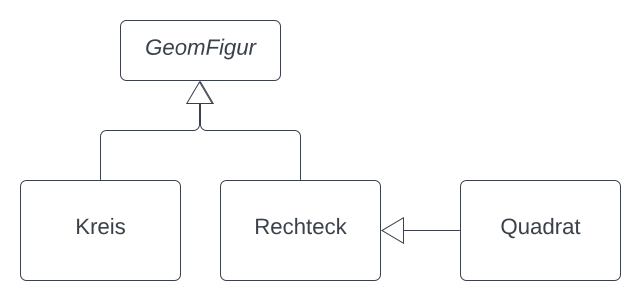
\includegraphics[
        width=8cm,
        keepaspectratio,
    ]{chapters/OOP/img/figur}
    \caption{Vererbungshierarchie der Klasse \textit{GeomFigur} und ihrer Subklassen.}
    \label{fig:figur}
\end{figure}


\noindent
Eine Klasse \code{FigurenFabrik} sei folgendermaßen gegeben:


\begin{minted}[mathescape,
    gobble=2]{java}
    class FigurenFabrik {

        /**
         * Erzeugt ein neues Quadrat mit der spezifizierten Seitenlänge.
         *
         * @param seitenLaenge die spezifizierte Seitenlänge.
         */
        public Quadrat erzeugeQuadrat(double seitenLaenge) {
            return new Quadrat(seitenLaenge);
        }
    }
\end{minted}\\

\noindent
Eine Klasse, die von \code{FigurenFabrik} erbt und \code{erzeugeQuadrat} überschreiben möchte,
muss sicherstellen, dass das von der Methode zurückgelieferte Objekt auch tatsächlich ein \code{Quadrat} ist.\\

\noindent
Hierzu darf der Rückgabetyp nicht allgemeiner sein. `Allgemeiner` bedeutet in diesem Fall: Typ \code{Rechteck} oder \code{Figur}.\\

\noindent
Ansonsten würden Zugriffe auf (vererbbare) spezifische Eigenschaften der Klasse \code{Quadrat} mit den zurückgelieferten Objekten zu Fehlern führen.
Der Compiler verhindert dies bereits:

\begin{minted}[mathescape,
    gobble=2]{java}
    class KaputteFigurenFabrik extends FigurenFabrik {

        public Rechteck erzeugeQuadrat(double seitenLaenge) {
            return new Rechteck(seitenLaenge, seitenLaenge*2);
        }
    }

    public class FigurenMacher {

        public static void main(String[] args) {
            FigurenFabrik f = new FigurenFabrik();

            // bevor es zum Programmabsturz waehrend der Laufzeit
            // aufgrund eines Aufrufs einer nur in Quadrat bekannten
            // Methode kommt, bricht der Compiler den Uebersetzungsvorgang
            // bereits mit einem Fehler ab
            f.erzeugeQuadrat().spezifischeMethodeAusQuadrat();
        }

    }
\end{minted}\\

\noindent
Der vom Compiler ausgegebene Fehler weist auf die Inkompatibilität der Rückgabetypen hin:\\

\begin{minted}{text}
    return type Rechteck is not compatible with Quadrat.
\end{minted}\\

\noindent
Für \textbf{Kovarianz} (und in diesem Zusammenhang \textbf{Kontravarianz}) und formalere Herleitungen sei auf
\textit{Das Liskovsche Substitutionsprinzip}\footnote{``Wikipedia - Liskov substitution principle``: \url{https://en.wikipedia.org/wiki/Liskov_substitution_principle}} (\cite{Lis87})
sowie den ausführlichen Beitrag im englischsprachigen Wikipedia \footnote{
    ``Wikipedia - Covariance and Contravariance``: \url{https://en.wikipedia.org/wiki/Covariance_and_contravariance_(computer_science)}
} verwiesen.
